\documentclass[a4paper,12pt]{scrartcl}

\input{./preamble/packages.tex}
\newif\ifheader
\newif\iffooter

\newif\ifacronymspage
\newif\iftitlepage
\newif\iftitlepageqrcode

\newif\ifsoftwarepage
    \newif\ifsoftwarepagelineartechnology
    \newif\ifsoftwarepagemicrochipstudio
    \newif\ifsoftwarepagefreecad
    \newif\ifsoftwarepagedremeldigilabslicer

\newif\ifcompetencepage
\newif\ifobjectivepage
\newif\ifhintspage

\headerfalse
\footerfalse

\acronymspagefalse
\titlepagefalse
\titlepageqrcodefalse

\softwarepagefalse
    \softwarepagelineartechnologyfalse
    \softwarepagemicrochipstudiofalse
    \softwarepagefreecadfalse
    \softwarepagedremeldigilabslicerfalse

\competencepagefalse
\objectivepagefalse
\hintspagefalse

% Globale Parameter
\setlength{\parindent}{0pt} % Kein Einrücken am Anfang eines Absatzes
\newcommand{\documentAuthor}{R. GÄCHTER}

% Header-Parameter
\headertrue           % Header aktivieren
  \newcommand{\headerLogo}{./images/g.raf.png}
  \newcommand{\headerText}{\textbf{g.raf - engineering\\Earth - Universe 1337}\\\texttt{Department of Electronics/Informatics}}

% Footer-Parameter
\footertrue           % Footer aktivieren
  \newcommand{\footerAuthor}{\documentAuthor}
  \newcommand{\footerVersion}{1.0}

% Page-Parameter
\acronymspagetrue         % Acronyme aktivieren
\tableofcontentspagetrue  % Inhaltsverzeichnis aktivieren
\listoffigurespagetrue    % Abbildungsverzeichnis aktivieren
\listoftablespagetrue     % Tabellenverzeichnis aktivieren
\bibliographypagetrue     % Literaturverzeichnis aktivieren

% Titlepage-Parameter
\titlepagetrue                % Titelblatt aktivieren
\titlepageqrcodetrue          % QR-Code auf dem Titelblatt aktivieren
\blankpageaftertitlepagetrue  % Leerseite nach dem Titelblatt aktivieren
  \newcommand{\titleHeadline}{Projektarbeit\\Temp}
  \newcommand{\titleLogo}{./images/g.raf.png}
  \newcommand{\titleLogoWidth}{0.2}
  \newcommand{\titleLogoCaption}{Titelbild der Projektarbeit}
  \newcommand{\titleDescription}{Kurzbeschreibung des Projekts\\}
  \newcommand{\titleRepository}{https://github.com/0x007e/???}

% Competencepage-Parameter
\competencepagetrue   % Kompetenz-Seite aktivieren
  % +---------------+---------------+
  % |       A       | BBBBBBBBBBBB  |
  % |      A A      | B           B |
  % |     A   A     | B           B |
  % |    A     A    | BBBBBBBBBBBB  |
  % |   AAAAAAAAA   | B           B |
  % |  A         A  | B           B |
  % | A           A | BBBBBBBBBBBB  |
  % +---------------+---------------+
  % | DDDDDDDDDDDD  |  CCCCCCCCCCCC |
  % | D           D | C             |
  % | D           D | C             |
  % | D           D | C             |
  % | D           D | C             |
  % | D           D | C             |
  % | DDDDDDDDDDDD  |  CCCCCCCCCCCC |
  % +---------------+---------------+
  \def\categories{Elektronik,Firmware,Mechanik,Prototyping}
  \def\numberOfsubcategories{4}
  \def\subcategories{
         270/{Messtechnik,Diskrete Bauteile,Analog-/Digital-Schaltungen,Einbau und Inbetriebnahme von Mikrocontrollern},           %A
          90/{Konfigurieren,Erstellen von Programmen,Erweitern von Programmen,Entwickeln von Algorithmen},                         %B
         -90/{Montage,Bearbeitungskonturen,Spanende-/Spanlose-Bearbeitung,Computergestuetzte Bauteilfertigung und -bearbeitung},  %C
        -270/{Materialauswahl,Datenaufbereitung (Slicing),3D-Druck/Laser-Cutting,Modellierung},                                   %D
          0/{} % Für korrekte Darstellung notwendig
      }
  % Verwendete Unterkategorien
  \def\catAvalue{4}
  \def\catBvalue{3}
  \def\catCvalue{1}
  \def\catDvalue{2}
  % Optional verwendete Unterkategorien
  \def\catAOptionalvalue{0}
  \def\catBOptionalvalue{1}
  \def\catCOptionalvalue{1}
  \def\catDOptionalvalue{2}

% Objectivepage-Parameter
\objectivepagetrue        % Lernziel-Seite aktivieren

% Hintspage-Parameter
\hintspagetrue            % Dokumentenhinweise aktivieren

% Softwarepage-Parameter
\softwarepagetrue     % Software-Seite aktivieren
  \softwarepagelineartechnologytrue
  \softwarepagemicrochipstudiotrue
  \softwarepagefreecadtrue
  \softwarepagedremeldigilabslicertrue

\input{./preamble/tabular.tex}
\input{./preamble/commands.tex}

\ifheader
  \input{./preamble/header.tex}
\fi

\iffooter
  \ifoot{\footerAuthor}
\cfoot{\footerVersion}
\ofoot{\thepage{} von \pageref{LastPage}}

\fi

\ifacronymspage
  \newcommand{\setupacronyms}{%
  \acro{tht}[THT]{Through-Hole Technology}
  \acro{smd}[SMD]{Surface-Mounted Device}
  \acro{updi}[UPDI]{Unified Program and Debug Interface}
  \acro{isp}[ISP]{In-System Programming}
  \acro{jtag}[JTAG]{Joint Test Action Group}
  \acro{cnc}[CNC]{Computerized Numerical Control}
}
\fi

\ifcompetencepage
  \usepackage{etoolbox}
\usepackage{xstring}
\usepackage{float}

\newcounter{competenceTableCounter}

\newcommand{\showCompetenceTable}[1]{
  \def\competencePath{./pages/competences/#1.csv}
  
  \stepcounter{competenceTableCounter}

  \begin{table}[!ht]
    \renewcommand{\arraystretch}{1.3}
    \centering
    \begin{tabularx}{\textwidth}{|c|X|}
      \hline
      \rowcolor{gray!20}
      \multicolumn{2}{|c|}{\large\textbf{#1}} \\
      \hline
      \textbf{Unterkategorie} & \textbf{Beschreibung des Kompetenzbereichs} \\
      \hline
      \csvreader[
        head to column names,
        separator=semicolon,
        late after line=\\\hline
      ]{\competencePath}{}{
        \Unterkategorie & \Beschreibung
      }
    \end{tabularx}
    \caption{Kompetenzbereich #1 – Aufgeteilt nach Unterkategorien}
  \end{table}

  \ifnum\value{competenceTableCounter}=2
    \thispagestyle{empty}
    \newpage
    \setcounter{competenceTableCounter}{0} % Zähler zurücksetzen
  \fi
}
\fi

% ##########################################################################

\begin{document}

\selectlanguage{english}

\iftitlepage
  \input{./pages/titlepage.tex}
  \maketitle

  \thispagestyle{empty}
  \newpage

  \ifblankpageaftertitlepage
    ~
    \thispagestyle{empty}
    \newpage
  \fi
\fi

\ifcompetencepage
  \section*{Kompetenzbereiche}

Im Rahmen des Projekts werden die farbig hervorgehobenen Kompetenzbereiche gezielt vermittelt. Diese Inhalte sind fester Bestandteil des Lehrplans und stellen sicher, dass alle Lernenden die grundlegenden Kenntnisse und Fertigkeiten in den Bereichen Elektronik, Mechanik, Firmware und Prototyping erwerben. Welche Kompezenzbereiche im Projekt vermittelt werden, kann im Detail den nachfolgenden Tabellen entnommen werden.

\vspace{-10pt}

\begin{figure}[ht]
  \centering
  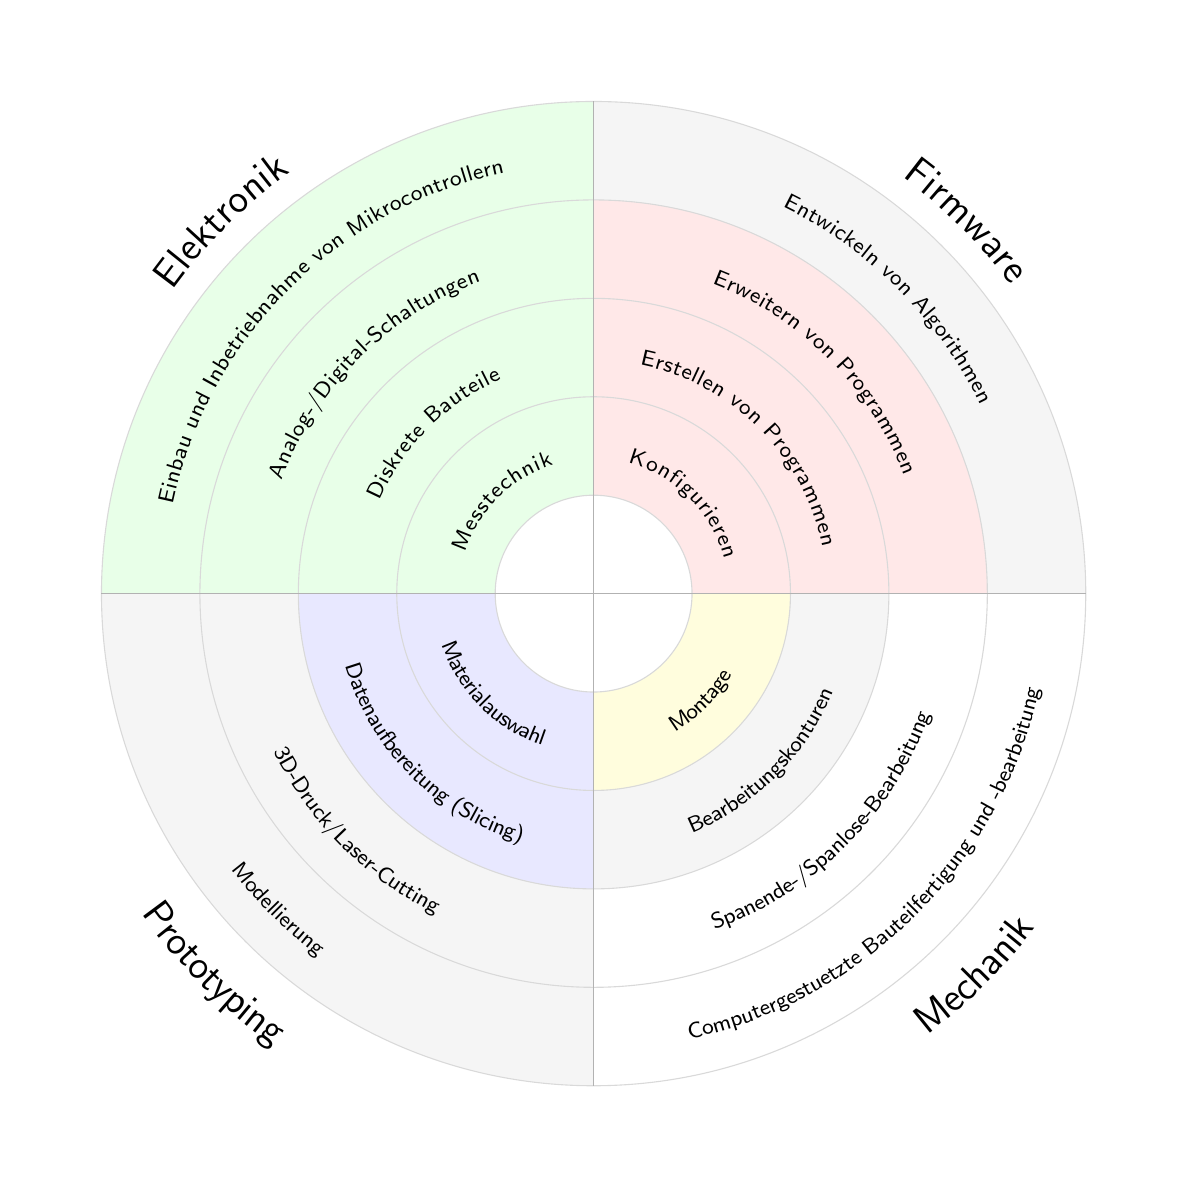
\begin{tikzpicture}[scale=1.25]
    % % Kreisradius
\usetikzlibrary{decorations.text}

\fill[green!20,opacity=0.45]  (0,0) -- (90:\catAvalue+1)  arc (90:180:\catAvalue+1)  -- cycle;
\fill[red!20,opacity=0.45]    (0,0) -- (0:\catBvalue+1)   arc (0:90:\catBvalue+1)    -- cycle;
\fill[yellow!30,opacity=0.45] (0,0) -- (270:\catCvalue+1) arc (270:360:\catCvalue+1) -- cycle;
\fill[blue!20,opacity=0.45]   (0,0) -- (180:\catDvalue+1) arc (180:270:\catDvalue+1) -- cycle;
\fill[white]    (0,0) -- (0:1)   arc (0:360:1)    -- cycle;


\ifnum\catAOptionalvalue>0
  \fill[gray!30,opacity=0.25]
    (90:\catAvalue+1) arc (90:180:\catAvalue+1) --
    (180:\catAvalue+1+\catAOptionalvalue) arc (180:90:\catAvalue+1+\catAOptionalvalue)
    -- cycle;
\fi

\ifnum\catBOptionalvalue>0
  \fill[gray!30,opacity=0.25]
    (0:\catBvalue+1) arc (0:90:\catBvalue+1) --
    (90:\catBvalue+1+\catBOptionalvalue) arc (90:0:\catBvalue+1+\catBOptionalvalue)
    -- cycle;
\fi

\ifnum\catCOptionalvalue>0
  \fill[gray!30,opacity=0.25]
    (270:\catCvalue+1) arc (270:360:\catCvalue+1) --
    (360:\catCvalue+1+\catCOptionalvalue) arc (360:270:\catCvalue+1+\catCOptionalvalue)
    -- cycle;
\fi

\ifnum\catDOptionalvalue>0
  \fill[gray!30,opacity=0.25]
    (180:\catDvalue+1) arc (180:270:\catDvalue+1) --
    (270:\catDvalue+1+\catDOptionalvalue) arc (270:180:\catDvalue+1+\catDOptionalvalue)
    -- cycle;
\fi

\pgfmathsetmacro{\maxval}{\numberOfsubcategories + 1}

% Hilfskreise
\foreach \r in {1,...,\maxval} {
  \draw[gray!30] (0,0) circle (\r);
}

% Achsen und Kategorien
\foreach \i [count=\idx from 1] in \categories {
  \draw[gray!60] (0,0) -- (90-90*\idx:\maxval);

  \pgfmathsetmacro{\startang}{450-180*\idx}
  \pgfmathsetmacro{\rr}{
    ifthenelse(\startang < 0, 5.75, 5.15)
  }
  \path[
    postaction={decorate},
    decoration={
      text along path,
      text={|\Large\sffamily|\i},
      text align={center},
      raise=1.0ex,
    }
  ]
  (\startang:\rr) arc (\startang:0:\rr);

}

\foreach \winkel/\liste in \subcategories{

  \pgfmathsetmacro{\rstart}{
    ifthenelse(\winkel < 0, 0.75, 0.25)
  }

  \foreach \text [count=\i from 1] in \liste {
    \pgfmathsetmacro{\r}{\rstart+\i}
    \path[
      postaction={decorate},
      decoration={
        text along path,
        text={|\footnotesize\sffamily|\text},
        text align={center},
        raise=1.0ex,
      }
    ]
    (\winkel:\r) arc (\winkel:0:\r);
  }
}

% \pgfmathsetmacro{\degree}{-90}
% \foreach \text [count=\i from 1] in {Flashen,Erstellen,Erweitern,Algorithmen} {
%   \pgfmathsetmacro{\r}{0.85 + \i}
%   \path[
%     postaction={decorate},
%     decoration={
%       text along path,
%       text={|\footnotesize\sffamily|\text},
%       text align={center},
%       raise=1.0ex,
%     }
%   ]
%   (\degree:\r) arc (\degree:0:\r);
% }

% \pgfmathsetmacro{\degree}{-270}
% \foreach \text [count=\i from 1] in {Slicintg,3D-Druck,Modellierung,Laser-Cutting} {
%   \pgfmathsetmacro{\r}{0.85 + \i}
%   \path[
%     postaction={decorate},
%     decoration={
%       text along path,
%       text={|\footnotesize\sffamily|\text},
%       text align={center},
%       raise=1.0ex,
%     }
%   ]
%   (\degree:\r) arc (\degree:0:\r);
% }

% \pgfmathsetmacro{\degree}{90}
% \foreach \text [count=\i from 1] in {Vorbearbeiten,Spanende-Bearbeitung,Spanlose-Bearbeitung,CNC} {
%   \pgfmathsetmacro{\r}{0.25 + \i}
%   \path[
%     postaction={decorate},
%     decoration={
%       text along path,
%       text={|\footnotesize\sffamily|\text},
%       text align={center},
%       raise=1.0ex,
%     }
%   ]
%   (\degree:\r) arc (\degree:0:\r);
% }

% \pgfmathsetmacro{\degree}{270}
% \foreach \text [count=\i from 1] in {Transistor,Analog,Digital,Mikrocontroller} {
%   \pgfmathsetmacro{\r}{0.25 + \i}
%   \path[
%     postaction={decorate},
%     decoration={
%       text along path,
%       text={|\footnotesize\sffamily|\text},
%       text align={center},
%       raise=1.0ex,
%     }
%   ]
%   (\degree:\r) arc (\degree:0:\r);
% }

  \end{tikzpicture}
  \caption{Darstellung der Kompetenzbereiche in einem Radardiagramm}
  \label{fig:kompetenzbereiche-radardiagramm}
\end{figure}

Die grau markierten (vertieften) Kompetenzbereiche können im Projekt ebenfalls bearbeitet werden. Das abarbeiten vertiefter Kompetenzbereiche ist freiwillig und kann auch (sofern möglich) außerhalb der regulären Unterrichtszeit stattfinden. Das abarbeiten vertiefter Kompetenzen sichert dem Lernenden zusätzliche Punkte im Feedback der Übung. Die grau markierten Bereiche zum vertieften Kompetenzerwerb sind im Projektverlauf deutlich gekennzeichnet.

\thispagestyle{empty}
\newpage

\renewcommand{\do}[1]{\showCompetenceTable{#1}}
\expandafter\docsvlist\expandafter{\categories}


  \thispagestyle{empty}
  \newpage
\fi

\ifobjectivepage
  \section*{Lernziele}

Die nachfolgenden Lernziele orientieren sich an den Taxonomiestufen nach Bloom und decken ein breites Spektrum von Wissenserwerb über Analyse und Bewertung bis hin zur Entwicklung eigener Lösungen ab. So wird sichergestellt, dass die Schüler:innen sowohl fachliches Know-how als auch anwendungsorientierte Kompetenzen erwerben.

Die Schüler:innen \ldots

\begin{itemize}
  \csvreader[
    head to column names,
  ]{./pages/objectives/objectives.csv}{}{
    \item \Kompetenz
  }
\end{itemize}

  \thispagestyle{empty}
  \newpage
\fi

\ifhintspage
  \section*{Hinweise zum Dokument}

Dieses Dokument beinhaltet Felder mit verschiedenen Funktionen. Eine kurze Erklärung 
soll Missverständnisse vorbeugen und das Bearbeiten des Dokuments vereinfachen. 

\begin{table}[!ht]
    \renewcommand{\arraystretch}{1.3}
    \centering
    \begin{tabularx}{\textwidth}{|M{0.85cm}|X|}
        \hline
        \rowcolor{gray!20}
        \csvreader[
            head to column names,
            separator=semicolon,
            late after line = \\\hline\rowcolor{gray!20}
        ]{./pages/hints/hints.csv}{}{
            \raisebox{-.25\height}{\includesvg[height=0.55cm]{./symbol/\Bild}} & \textbf{\Titel} \\
            \hline
            \multicolumn{2}{|p{\dimexpr\textwidth-2\tabcolsep}|}{\Beschreibung}
        }
    \end{tabularx}
    \caption{Kategorien der Dokumentenhinweise}
\end{table}


  \thispagestyle{empty}
  \newpage
\fi

\ifsoftwarepage
  \newcounter{softwaretnotecounter}

\section*{Benötigte Software}
\begin{table}[!ht]
  \renewcommand{\arraystretch}{1.3}
  \centering
  \begin{threeparttable}
    \begin{tabularx}{\linewidth}{|M{2.4cm}|M{2.2cm}|X|}
      \hline
      \rowcolor{gray!20}
      \textbf{Abbildung\tnote{*}} & \textbf{Name} & \textbf{Beschreibung} \\
      \hline
\ifsoftwarepagelineartechnology
      \stepcounter{softwaretnotecounter}
      \includesvg[width=1.6cm]{./logo/linear_technology} &
      LT-Spice\tnote{(\thesoftwaretnotecounter)} &
      Simulationssoftware für elektronische Schaltungen, weitverbreitet zum Entwurf und Testen von Schaltungen.\\
      \hline
\fi
\ifsoftwarepagemicrochipstudio
      \stepcounter{softwaretnotecounter}
      \includesvg[width=1.6cm]{./logo/microchip} &
      Microchip Studio\tnote{(\thesoftwaretnotecounter)} &
      Entwicklungsumgebung (IDE) zur Programmierung von Mikrocontrollern, insbesondere AVR und ARM.\\
      \hline
\fi
\ifsoftwarepagefreecad
      \stepcounter{softwaretnotecounter}
      \includesvg[width=0.65cm]{./logo/freecad} &
      FreeCAD\tnote{(\thesoftwaretnotecounter)} &
      Open-Source CAD-Software für 3D-Modellierung, geeignet für technische Konstruktionen und Design.\\
      \hline
\fi
\ifsoftwarepagedremeldigilabslicer
      \stepcounter{softwaretnotecounter}
      \includesvg[width=1.6cm]{./logo/dremel} &
      Dremel 3D DigiLab Slicer\tnote{(\thesoftwaretnotecounter)} &
      Software zum Vorbereiten und Slicen von 3D-Druck-Modellen, speziell für Dremel 3D-Drucker optimiert.\\
      \hline
\fi
    \end{tabularx}
    \caption{Softwarekomponenten für das Projekt}
    \label{tab:software-programme}
    \begin{tablenotes}
      \footnotesize
      \item[*] Die abgebildeten Logos sind markenrechtlich geschützte Symbole. Sie werden in dieser Dokumentation ausschließlich zur Identifikation der jeweiligen Softwareprodukte verwendet, ohne Werbeabsicht.
      \item[~]
\setcounter{softwaretnotecounter}{0}
\ifsoftwarepagelineartechnology
      \stepcounter{softwaretnotecounter}
      \item[(\thesoftwaretnotecounter)] \url{https://www.analog.com/en/resources/design-tools-and-calculators.html}
\fi
\ifsoftwarepagemicrochipstudio
      \stepcounter{softwaretnotecounter}
      \item[(\thesoftwaretnotecounter)] \url{https://www.microchip.com/en-us/tools-resources/develop/microchip-studio}
\fi
\ifsoftwarepagefreecad
      \stepcounter{softwaretnotecounter}
      \item[(\thesoftwaretnotecounter)] \url{https://www.freecad.org/downloads.php}
\fi
\ifsoftwarepagedremeldigilabslicer
      \stepcounter{softwaretnotecounter}
      \item[(\thesoftwaretnotecounter)] \url{https://www.dremel.com/at/de/digilab/3d-druckersoftware}  
\fi
    \end{tablenotes}
  \end{threeparttable}
\end{table}

  \thispagestyle{empty}
  \newpage
\fi

\iflanguage{english}{
  \section*{Abstract}
}{
  \section*{Vorwort}
}

Die Geschichte der Kryptografie ist eng mit technischen Innovationen und gesellschaftlichen Ereignissen verflochten. Ein besonders eindrucksvolles Beispiel moderner Verschlüsselungstechnik ist die \texttt{Enigma-Maschine}\footnote{\url{https://de.wikipedia.org/wiki/Enigma_(Maschine)}}. Die \texttt{Enigma} wurde in den 1920er-Jahren vom deutschen Ingenieur \texttt{Arthur Scherbius} entwickelt und ursprünglich als kommerzielle Chiffriermaschine für Banken und Unternehmen angeboten \parencite{copeland2017}. Erst später erlangte sie internationale Bekanntheit, als das deutsche Militär ihre hohe Verschlüsselungskraft erkannte und die Maschine ab Ende der 1920er-Jahre zur geheimen Kommunikation einsetzte. Während des Zweiten Weltkriegs war die \texttt{Enigma} das Herzstück der deutschen Militärkommunikation. Die Wehrmacht, die Kriegsmarine und andere Einheiten verwendeten \texttt{Enigma-Maschinen}, um Nachrichten zu chiffrieren und so vor feindlichem Zugriff zu schützen. Die Komplexität des Systems sollte eine Entschlüsselung durch die Alliierten verhindern. Die Entzifferung der \texttt{Enigma} durch ein internationales Team von Codeknackern, darunter \texttt{Marian Rejewski} und später \texttt{Alan Turing} in Bletchley Park, gilt als Meilenstein der Kryptografiegeschichte. Ihre Arbeit trug maßgeblich dazu bei, den Verlauf des Krieges mitzugestalten und das Zeitalter der Computertechnik einzuleiten. Die \texttt{Enigma} arbeitete auf elektromechanischer Basis nach dem Prinzip eines \texttt{polyalphabetischen Substitutionsverfahrens}\footnote{\url{https://de.wikipedia.org/wiki/Polyalphabetische_Substitution}}.Die \texttt{Enigma} steht exemplarisch für die Herausforderungen und Möglichkeiten maschineller Verschlüsselung. Ihr Design macht deutlich, wie technische Innovation und mathematisches Verständnis zusammenwirken, um die Sicherheit von Informationen zu gewährleisten – ein Aspekt, der bis heute in der IT-Sicherheit relevant ist.

\thispagestyle{empty}
\newpage

\iftableofcontentspage
  % Gliederungstiefe bis subsubsection (Inhaltsverzeichnis)
  % \setcounter{tocdepth}{2}
  \tableofcontents

  \thispagestyle{empty}
  \newpage
\fi

\setcounter{page}{1}

\noindent\hfill\texttt{GAR@\today|\jobname.pdf}
\vspace{-25pt}

\section{Grundlagen}
Dies ist ein einfaches LaTeX-Dokument mit einer benutzerdefinierten Kopf- und Fußzeile auf Basis von \texttt{scrlayer-scrpage}.

\section{Elektronik}
Der Hauptinhalt beginnt hier. Du kannst in diesem Abschnitt deine Themen darstellen, Formeln integrieren oder Tabellen einfügen.

\section{Prototyping}
Dies war ein Beispiel für ein grundlegendes LaTeX-Template mit Kopf- und Fußzeilen.

\section{Firmware}
Dies war ein Beispiel für ein grundlegendes LaTeX-Template mit Kopf- und Fußzeilen.

\section{Mechanik}
Dies war ein Beispiel für ein grundlegendes LaTeX-Template mit Kopf- und Fußzeilen.

\section{Reflektion}
Dies war ein Beispiel für ein grundlegendes LaTeX-Template mit Kopf- und Fußzeilen.

\section{Feedback}
Dies war ein Beispiel für ein grundlegendes LaTeX-Template mit Kopf- und Fußzeilen.

\newpage

\ifacronymspage
  \section*{Abkürzungsverzeichnis}

\begin{acronym}[JTAG]
  \setupacronyms
\end{acronym}

  \thispagestyle{empty}
  \newpage
\fi

\iflistoffigurespage
  \listoffigures
\fi

\iflistoftablespage
  \listoftables
\fi

\iflistoffigurespage
  \thispagestyle{empty}
  \newpage
\else
  \iflistoftablespage
    \thispagestyle{empty}
    \newpage
  \fi
\fi


\ifbibliographypage
  \printbibliography[title={Literaturverzeichnis}]
  \thispagestyle{empty}
\fi
\end{document}